%==== Document Setup (usthesis)======================================

\documentclass[report, 12pt,oneside,openany,a4paper, a5block a4paper,afrikaans,english]{usthesis}
\usepackage[hmargin={10mm,10mm},vmargin={20mm,20mm}]{geometry}
\usepackage{float}
%
% PLEASE read the USthesis documentation for the class options
% and how to set line and paragraph spacing
%

%==== Language setup ================================================
 \usepackage[latin1]{inputenc}%................... Recognizes �, �, etc
 \usepackage{babel}%.............................. Language setup

%==== Math setup ====================================================
 \usepackage{amsmath}%............................ Advanced math (before fonts)
 %\usepackage{amssymb}%............................ AMS Symbol fonts

%==== Font setup (default is Computer Modern) =======================
 \usepackage[T1]{fontenc}%........................ Type 1 fonts
 \usepackage{textcomp}%........................... Additional text character
 \usepackage{bm}%................................. Bold math symbols (after fonts)

%==== Ref's, Bib's and Nomencl ======================================
 \usepackage{usnomencl}%.......................... List of symbols (in usthesis pack)
 \usepackage{usbib}%.............................. Bibliography    (in usthesis pack)
    \bibliographystyle{usmeg-a}
    \renewcommand\bibfont{\small}

    %% For usmeg-a, the bib is a list of references. If you
    %% are using usmeg-n comment out the following lines
    \addto{\captionsafrikaans}{\renewcommand{\bibname}{Lys van Verwysings}}
    \addto{\captionsenglish}{\renewcommand{\bibname}{List of References}}

%==== Graphics and Color ============================================
\usepackage{graphicx}%........................... Graphicx loaded in usthesis
\usepackage{color}%.............................. Color setup

%==== Additional USthesis packages ==================================

\usepackage{ussummary}%.......................... Mech Eng summary page (in usthesis pack)

%==== Local Defs ====================================================
\makeatletter

%
% Please insert user defined commands here
% and NOT in the document itself!
%

\makeatother
%==== Title Page ====================================================

\title{Mininet Network Emulator}

\author{I.T.\ de Villiers}
       {Ignatius Thomas de Villiers\\
           17502292}

\subject{Project (e) 448}
        {Department Electrical and  Electronic Engineering,\\Stellenbosch University,\\Private Bag X1, Matieland 7602.}

\ReportDescript{Dissertation Report}

\address{Department Electrical and  Electronic Engineering,\\Stellenbosch University,\\Private Bag X1, Matieland 7602.}

\studyleader{Dr H.A.\ Engelbrecht}

\setdate{11}{2016}



%====================================================================%
%                 T H E   M A I N   D O C U M E N T                  %
%====================================================================%
\begin{document}

\frontmatter%========================================================

\TitlePage
\CopyrightPage
\include{verklaring}
\chapter{Acknowledgements}

I would like to express my deepest  appreciation to all those who provided me the possibility to complete this report. A special 
griatitude I give to my study leader Dr. H.A. \ Engelbrecht, whose contribution in simulating suggestions,  project coordination and guidance
helped me to write this report\\\\
Furthermore I would Like to give my gratitude to Mr I.D. \ de Villiers (Software Development Engineer, Amazon), who's contribution in terms of software structure guidance and the reviewing of all functional code, has helped me to complete the Mininet Network Emulator Tool.

\include{opsomming}
\include{uittreksel}
\tableofcontents
\listoffigures
\listoftables
%\include{nomenkl}

\mainmatter%=========================================================

\numberwithin{equation}{section}%(from amsmath)
\numberwithin{figure}{section}  %
\numberwithin{table}{section}   %

 \graphicspath{ {GUI/} }
\chapter{Introduction}
\section{Background}

This project was initiated by Dr H.A.\ Engelbrecht to develop a lab tool with which a person can test
a topology's performance under various network conditions without having to set up the network\\

\section{Literature Study}
\section{Aims and Objectives}

\begin{enumerate}
\item Simulate various custom topologies under  user-defined network conditions.
\begin{enumerate}
\item Using all virual components (Hosts, switches, etc) over the emulated network.
\item Using some real components over the emulated network.
\end{enumerate}
\item Create a easy-to-use Graphical User Interface, to allow customization of:
\begin{enumerate}
\item Topology
\item Network conditions
\end{enumerate}
\item Allow user to save custom topologies
\item Test all custom topologies under same conditions
\item Stream a video and/or DHCP server over the network and to see accurate results
\item Create an accurate network simulator capable of:
\begin{enumerate}
\item Setting up network with it's conditions
\item Streaming over the network
\item Alternative testing of network conditions
\end{enumerate}
\end{enumerate}\newpage
\section{Graphical User Interface}
To ensure that the user gets the most out of the Mininet Network Emulator tool, it is important 
to allow the user to specify the network Topology and set various network conditions, like \textit{bandwidth}, \textit{delay},
\textit{Packet loss} and \textit{jitter}. When the program is Started the first window that appears, is the \textit{Working Directory} Window, shown in Figure 1.4.1. This window prompts the user to enter a save location for the topology they are about to create.  As seen in figure 1.4.1, the main window consists of three widget frames, namely the \textbf{\textit{Hosts Widget}},  \textbf{\textit{Switches Widget}} and the  \textbf{\textit{Links Widget}}. Each of these widgets allow the user to add hosts and switches and to customize the link parameters for each host to a switch. Figure1.4.2 shows the inner workings of the GUI.
\begin{figure}[H]
    \centering
    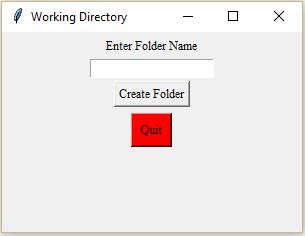
\includegraphics[scale=0.8]{Directory}
    \caption{Initial Window on starting the Mininet Network Emulator}
\end{figure}
\begin{figure}[H]
    \centering
    \textbf{Mininet Network Emulator GUI}\par\medskip
    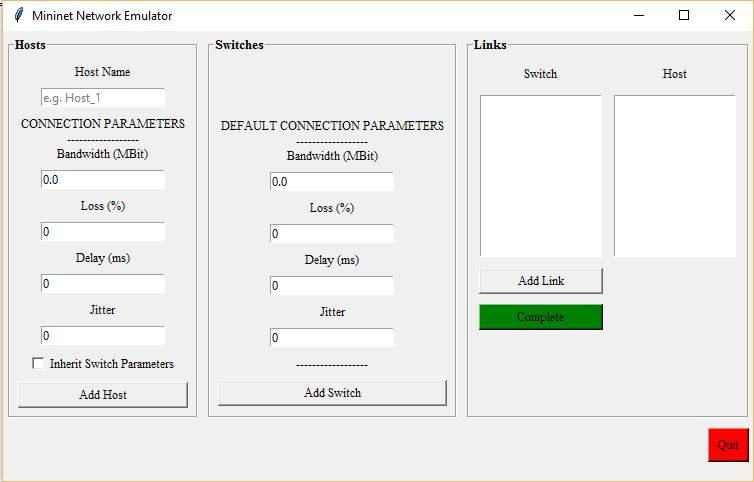
\includegraphics[scale=0.5]{Entire_window}
    \caption{Mininet Network Emulator GUI Frame}
\end{figure}
\begin{figure}[H]
    \centering
    \includegraphics[scale=0.7]{GUIflow}
    \caption{GUI flow chart - showing all steps the during the creation of a topology}
\end{figure}

\subsection{Hosts Widget}
The Host widget essentialy, as seen in Figure 1.4.3, allows the user to add host entities to the network. The user can customize the Host ID/Host Name by entering a name into the first textfield. In the case that the user leaves the textfield blank, a default name \textit{'h1', 'h2', 'h3', etc} will be used. The user can also add connection parameters/non-idealities for each individual Host, \textit{bandwidth}, \textit{delay}, \textit{Packet loss} and \textit{jitter}, to simulate a real life connection. Value testing prevents the user from entering invalid parameters into textfields, like text and other ascii values, to ensure only valid entries are saved. Default values for all the connection parameters are 0. The radio button \textbf{\textit{Inherit Switch parameters}}, instantly changes the Host link parameters to inherit the switch's connection parameters when it is selected. When the \textbf{\textit{Add Host Button} }is pressed, the host name and all it's connection parameters are written into a text file \textit{'hosts.txt'}, as seen in Figure 1.4.3, which is then later used to create mininet objects- this will be discussed later in this document.\\
\begin{figure}[H]
\centering
\begin{minipage}{.5\textwidth}
  \centering
  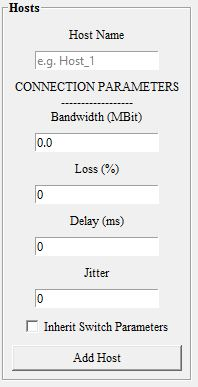
\includegraphics[width=.4\linewidth]{Hosts}
  \caption{Hosts widget, which allows the user to add Hosts to the network, and customize it's connection parameters}
  \label{fig:test1}
\end{minipage}%
\begin{minipage}{.5\textwidth}
  \centering
  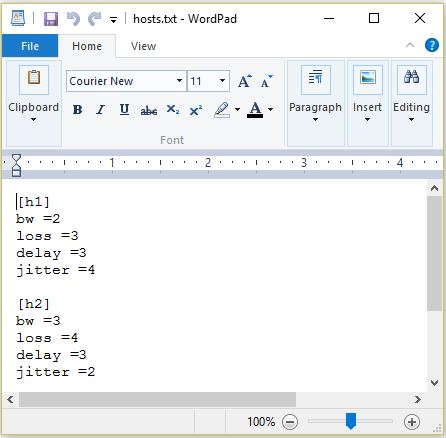
\includegraphics[width=.8\linewidth]{hosts_txt}
  \caption{Example of created Hosts text file}
  \label{fig:test2}
\end{minipage}
\end{figure}

\subsection{Switches Widget}
The Switches widget, as seen in Figure 1.4.5, essentialy allows the user to add switch entities to the network. A default name \textit{'S1', 'S2', S3', etc} is automatically assigned to each switch entity. The user can also add connection parameters/non-idealities for each individual switch, \textit{bandwidth}, \textit{delay}, \textit{Packet loss} and \textit{jitter}, which is similar to the Host connection parameters but are only used when the user decides to add baseline parameters, which a link will inherit in the case that the Host connecting to the switch's parameters are 0. Value testing prevents the user from entering invalid parameters into textfields, like text and other ascii values, to ensure only valid entries are saved. Default values for all the connection parameters are 0. When the \textbf{\textit{Add Switch Button}} is pressed, the switch name an all it's connection parameters are written into a text file \textit{'switches.txt'}, as seen in Figure, which is then later used to create mininet objects- this will be discussed later in this document.\\
\begin{figure}[H]
\centering
\begin{minipage}{.5\textwidth}
  \centering
  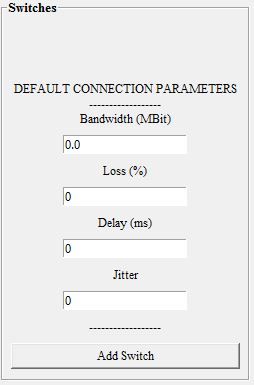
\includegraphics[width=.5\linewidth]{Switches}
  \caption{Switches widget, which allows the user to add Switches to the network, and customize the default connection parameters}
  \label{fig:test1}
\end{minipage}%
\begin{minipage}{.5\textwidth}
  \centering
  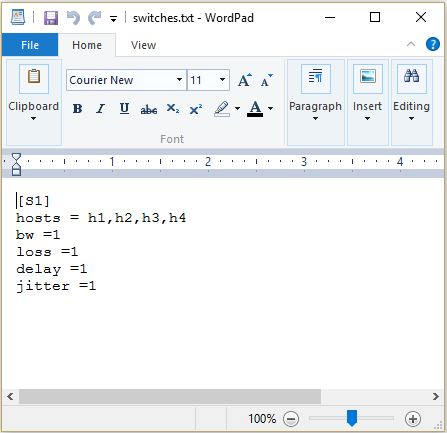
\includegraphics[width=.8\linewidth]{switches_txt}
  \caption{Example of created Switches text file}
  \label{fig:test2}
\end{minipage}
\end{figure}

\subsection{Links Widget}
The Links widget essentialy allows the user to link network entities, namey $x$ amount of hosts to 1 switch. As shown in figure 1.4.7, two Listboxes are used, the Host-listbox and the Switches-listbox, the user selects one or more hosts from the first listbox and then selects the switch they want to connect the hosts to. After they have decided which links they want make, the user can then click the \textbf{\textit{Add Link Button}} which will then save the Hosts connected to a specific switch and save it to the textfile \textit{'switches.txt'}, as seen in Figure 1.4.6, to indicate which entities are connected to one another.
\begin{figure}[H]
    \centering
    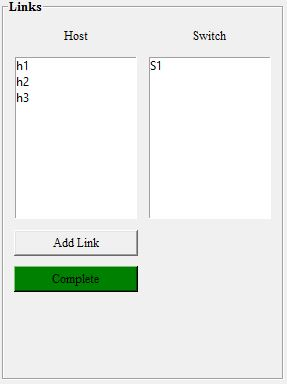
\includegraphics[scale=0.7]{Links}
    \caption{Links widget}
\end{figure}\newpage

\subsection{Visuals Widget}
Once all the Network Entities are added and the necassary links were created, the Visuals widget, in the form of a tkinter canvas widget, allows the user the graphically see the Network. This widget could come in handy when very large topologies are created - this will allow the user to review his work. The user is also able to move the objects around within the tkinter canvas, in order to created and test various setups. In Figure 1.4.8 we see the visuals created for a basic of a Star Topology example.
\begin{figure}[H]
    \centering
    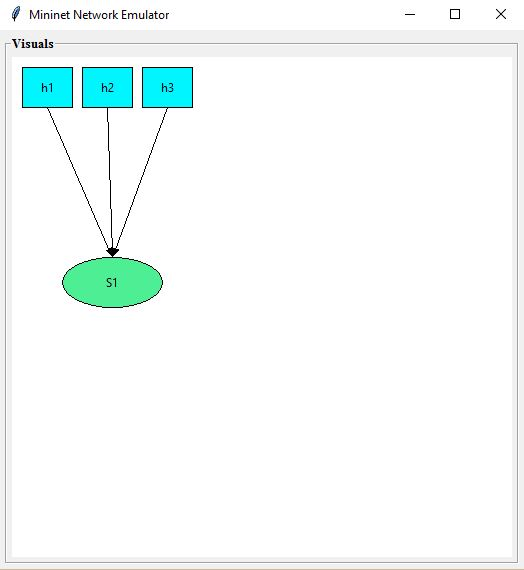
\includegraphics[scale=0.5]{Visuals}
    \caption{Example: Three Hosts, one Switch, star topology \textbf{\textit{Complete Button}} is pressed. }
\end{figure}

%\include{Chp-2}
%\include{Chp-3}

\appendix%===========================================================

 \chapter{Konsepte Gegenereer}
\section{Konsep I}
\section{Konsep II}

%\include{App-B}
%\include{App-C}

\backmatter%=========================================================

\bibliography{USbibsample}

\end{document}
